
The constitutive framework developed in Section \ref{sec:constitutive equations} is formulated from a generalized continuum perspective, rendering it applicable to a wide class of responsive materials. In the specific context of electroactive polymers (EAPs), a rich body of literature has addressed isolated physical phenomena—namely purely mechanical, thermal, or electrical behaviours \cite{Hossain2012visco,Dippel2015}—as well as dual-field interactions \cite{Liao_Mokarram2020,Alkhoury2022} and fully coupled, thermo-electro-mechanical responses \cite{Mehnert2021a,Sheng2012,Qin2023}. Driven by the availability of comprehensive experimental datasets, the widely utilized acrylic elastomer VHB is selected herein as a benchmark material to validate the proposed theoretical formulation. 

This calibration process extends beyond routine parameter optimization; it serves as a rigorous means to validate the choice of underlying mechanical models—such as the configuration of the Maxwell branches—and to verify the predictive capability of the thermodynamically consistent coupling functions. Ultimately, the objective of this section is to demonstrate the robust performance of the proposed framework, establishing a systematic characterization methodology that can be readily extended to other electro-thermo-viscoelastic smart materials.


\subsection{Data availability and experimental characterization}
\label{sec:experimental_data}

To inform and validate the multi-field constitutive model, a comprehensive review and classification of experimental data from the existing literature was conducted. The selected experimental landscape spans a broad temperature range from -20°C to 80°C and encompasses both isolated single-physics tests and highly coupled multi-field protocols. These data streams are systematically categorized in Table \ref{tab:experiment_sources} and visually summarized across distinct physical regimes in Fig. \ref{fig:selected_experiments}.


\subsubsection{Experimental data description}

\begin{table}[htb]
\centering
\caption{Types, operational regimes, and literature sources of the experimental data used for calibration.}
\label{tab:experiment_sources}
\begin{tabular}{@{}lll@{}}
\toprule
Experiment Type & Description & References \\
\midrule
Thermal    & Differential scanning calorimetry (DSC)   & \cite{Dippel2015,Sheng2012} \\ \addlinespace
Electrical & Broadband dielectric spectroscopy (BDS)   & \cite{Sheng2012} \\ \addlinespace
\multirow{3}{*}{Mechanical}%
           & Quasi-static loading                      & \cite{Hossain2012visco} \\
           & One-cycle loading-unloading               & \cite{Hossain2012visco} \\
           & Constant stretch creep                    & \cite{Hossain2012visco,Alkhoury2022} \\ \addlinespace
\multirow{3}{*}{Thermo-mechanical}%
           & Quasi-static loading                      & \cite{Liao_Mokarram2020} \\
           & One-cycle loading-unloading               & \cite{Liao_Mokarram2020,Alkhoury2022} \\
           & Constant stretch creep                    & \cite{Liao_Mokarram2020,Alkhoury2022} \\ \addlinespace
Thermo-Electro-Mechanical%
           & One-cycle loading-unloading               & \cite{Mehnert2021a,Qin2023} \\
\bottomrule
\end{tabular}
\end{table}

\paragraph{Thermal Characterization}
The baseline thermal response is characterized via Differential Scanning Calorimetry (DSC), executed under standardized testing protocols \cite{Hohne2003_DSC}. By subjecting the polymer specimen to a controlled thermal ramp at a constant rate, the resulting heat flux measurements isolate the temperature-dependent specific heat capacity in the absence of mechanical or electrical fields (see Fig. \ref{fig:selected_experiments}a).

\paragraph{Electrical Characterization}
The small-strain dielectric permittivity is identified by means of Broadband Dielectric Spectroscopy (BDS) \cite{Kremer2003_BDS}. These tests measure the material dielectric constant across a wide spectrum of frequencies under a prescribed alternating electric field (Fig. \ref{fig:selected_experiments}b), assuming the specimen remains at its thermodynamic reference state (undeformed and at room temperature).

\paragraph{Mechanical and Coupled Characterization} 
Unlike the standalone thermal and electrical tests, multi-field mechanical testing typically lacks universally standardized protocols, particularly when exploring the coupled viscoelastic response of EAPs. The uniaxial mechanical testing matrix analysed herein encompasses quasi-static loading, single- and multi-step creep histories, and cyclic loading-unloading profiles. These tests record the nominal (first Piola-Kirchhoff) stress as a function of stretch, and are systematically repeated across different ambient temperatures (Figs. \ref{fig:selected_experiments}c and \ref{fig:selected_experiments}d) and applied electrostatic potentials. While the creep tests isolate the long-term, asymptotic hyperelastic equilibrium state of the polymer, the cyclic loading-unloading configurations capture the rate-dependent viscous dissipation mechanism.


\begin{figure}[htb]
  \centering
  \begin{subfigure}{0.45\textwidth}
    
\includegraphics[width=\textwidth]{figures/qualitative_experim_calorimetry.pdf}
    \caption{DSC tests, extracted from \cite{Dippel2015}}
    \label{fig:selected_experim_dsc}
  \end{subfigure}
  \hspace{1em}
  \begin{subfigure}{0.45\textwidth}
    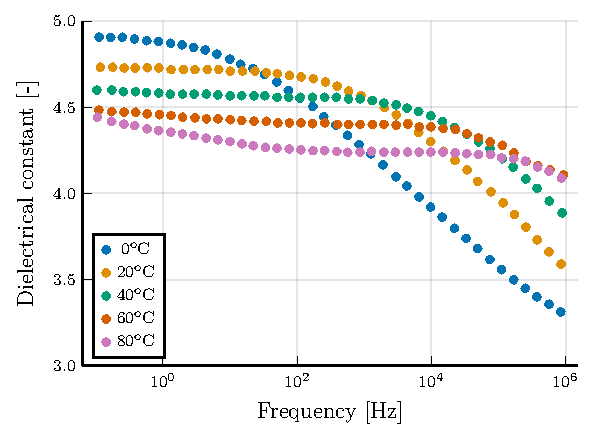
\includegraphics[width=\textwidth]{figures/qualitative_experim_dielectrical.pdf}
    \caption{BDS tests, extracted from \cite{Sheng2012}}
    \label{fig:selected_experim_bds}
  \end{subfigure}
  \vspace{1em}
  \begin{subfigure}{0.45\textwidth}
    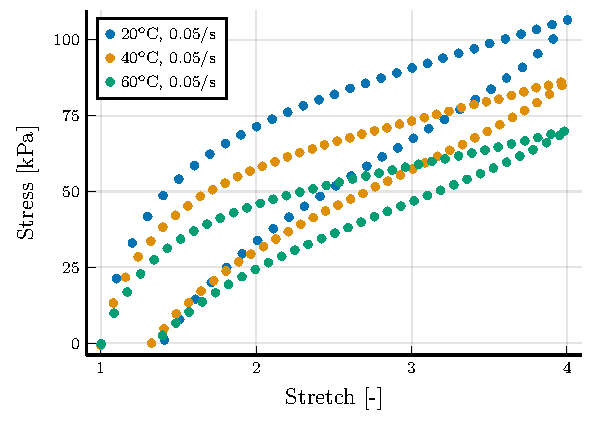
\includegraphics[width=\textwidth]{figures/qualitative_experim_one_cycle.pdf}
    \caption{Loading-unloading tests, extracted from \cite{Liao_Mokarram2020}}
    \label{fig:selected_experim_load}
  \end{subfigure}
  \hspace{1em}
  \begin{subfigure}{0.45\textwidth}
    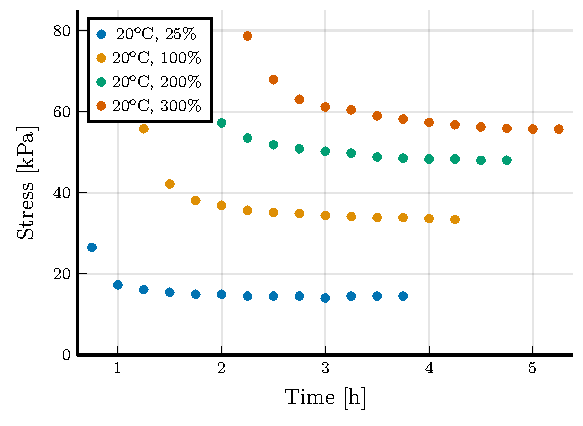
\includegraphics[width=\textwidth]{figures/qualitative_experim_creep.pdf}
    \caption{Creep tests, extracted from \cite{Liao_Mokarram2020}}
    \label{fig:selected_experim_creep}
  \end{subfigure}
  \caption{Visualization of selected experimental tests showing the thermo-electro-mechanical response of the material.}
  \label{fig:selected_experiments}
\end{figure}


\subsubsection{Data selection and curation}
\label{subsubsec:data_curation}

Discrete data points were extracted from the graphical records of the cited original publications using the digitized coordinate software \textit{WebPlotDigitizer} \cite{webplotdigitizer}. The raw extracted data arrays were filtered, post-processed for baseline uniformity, and organized into an open-access, consolidated repository to ensure complete reproducibility. This curated dataset is available in the electronic \textbf{Supplementary Material}.


\subsubsection{Evaluation of data consistency}
\label{subsubsec:data_consistency}

A primary challenge in calibrating multi-physics constitutive models for elastomers is the significant scatter and apparent lack of consistency in cross-laboratory data. For instance, identical mechanical tests executed on the nominal same material under matched temperature, strain rate, and stretch limits can exhibit inter-laboratory stress discrepancies of up to 50\%. This experimental variance similarly affects reported thermal and electrical properties.

Several microstructural and manufacturing factors contribute to this observed scatter:
\begin{enumerate}
    \item \emph{Commercial optimization intent:} VHB polymers are manufactured primarily as industrial adhesive tapes rather than structural engineering elastomers; hence, quality control prioritizes the properties aligned with its intended use.
    \item \emph{Thickness-dependent curing:} The polymer is supplied in various nominal thicknesses, which may alter the curing kinetics during production, yielding distinct underlying cross-link densities.
    \item \emph{Batch-to-batch variability:} Engineering tolerances for continuum stiffness parameters are not tightly restricted by manufacturers, leading to noticeable deviations between production lots.
\end{enumerate}


While these variations raise meaningful questions regarding material uncertainty and error propagation, a detailed statistical analysis of batch variability falls outside the scope of this investigation. To assess the fundamental suitability of the proposed continuum framework to capture coupled electro-thermo-viscoelastic behaviours, a consistent, kinematically compatible subset of data has been selected for the sequential parameter optimization detailed in section \ref{sec:optim_framework}.



\subsection{Reduced constitutive equations for homogeneous deformation}
\label{sec:reduced_equations}

To bridge the general three-dimensional continuum theory established in section \ref{sec:constitutive equations} with the predominantly scalar nature of the experiments detailed in section \ref{sec:experimental_data}, the governing multi-field equations must be specialized for homogeneous deformation states. For a given experimental protocol $k$, the gathered data can be formalized as a discrete set of observations pairing a vector of independent, controllable state variables $\vect{x}$ with a measurable scalar response $y$. Consequently, for each sampling point $i \in \{1, \dots, N_k\}$, the experimental track is represented by the dataset:
%
\begin{equation}
    \mathcal{D}_k = \left\{ (\vect{x}_i, y_i) \right\}_{i=1}^{N_k}
\end{equation}
%
where $\vect{x}_i$ denotes the localized thermodynamic and kinematic control state —encompassing specific combinations of longitudinal stretch $\lambda$, temperature $\theta$, time $t$, or nominal electric potential $V$— while $y_i$ represents the corresponding physical observable, namely the specific heat capacity $c_v$, the primary longitudinal component of the first Piola-Kirchhoff stress $P_{11}$, or the effective dielectric permittivity $\varepsilon$.

This scalar-valued operational framework necessitates a two-fold reduction of the fully coupled 3D field equations. First, the deformation gradient and field operators must be structurally constrained to uniquely define the independent control vector $\vect{x}$ based on the boundary conditions of each test configuration. Second, the corresponding energy-conjugate stress and multi-field response measures must be analytically derived via thermodynamic differentiation of the free energy density $\Psi$, providing the scalar model predictions $y_{\text{pred}}(\vect{x})$ required for the inverse optimization problem.



\subsubsection{Kinematics and thermal expansion}

\paragraph{Volumetric deformation and stress-free Jacobian}

During both the differential scanning calorimetry (DSC) and the unconstrained thermo-mechanical configurations, the polymer is subjected to uniform temperature variations that induce finite volumetric changes via isotropic thermal expansion. Because the specimens expand freely without external mechanical confinement, the hydrostatic pressure $p$ —defined as the thermodynamic force conjugate to the total volume ratio or Jacobian $J$— must vanish. Setting the derivative of the purely volumetric component of the free energy density $\bar{\Psi}$ in \eqref{eqn:volumetric_free_energy} with respect to $J$ to zero yields the thermodynamic equilibrium condition:
%
\begin{equation} \label{eqn:thermal_Jacobian}
    p = \frac{\partial\bar\Psi}{\partial J} = 0 \quad\Longrightarrow\quad
    J(\theta) = 1 + 3\alpha\frac{\theta_R}{\bar\gamma+1}
    \left(\left(\frac{\theta}{\theta_R}\right)^{\bar\gamma+1} - 1\right).
\end{equation}


\paragraph{Uniaxial stretch kinematics}

For a baseline, purely mechanical configuration evaluated under isothermal and uncharged conditions, the deformation state simplifies to an unconstrained uniaxial tension profile. Assuming an incompressible material response for the baseline elastomer, the resulting isochoric kinematic mapping is defined by the deformation gradient:
%
\begin{equation}
  \F_M = \begin{bmatrix}
    \lambda & 0 & 0 \\
    0 & \lambda^{-1/2} & 0 \\
    0 & 0 & \lambda^{-1/2}
  \end{bmatrix},
\end{equation}
%
where $\lambda \ge 1$ denotes the principal stretch imposed along the primary longitudinal axis.


\paragraph{Thermally coupled uniaxial state}

To accurately model the thermo-mechanical tests reported in \cite{Liao_Mokarram2020,Alkhoury2022}, the kinematic framework must account for the specific sequence of thermal conditioning and mechanical clamping. The experimental protocol is described as follows:
\begin{displayquote}
  First, the specimens were placed inside the chamber and conditioned at the target temperature for fifteen minutes to achieve thermal homogeneity across the \si{0.5}{mm} thickness. Crucially, the specimens were mounted onto the grippers only after this thermal stabilization period. The protective silicon paper was then removed gently to ensure the test initiated without any pre-tension.  
\end{displayquote}
This protocol dictates that the laboratory reference configuration —corresponding to an adjusted longitudinal stretch of $\lambda=1$ and zero nominal stress— is established after the material has undergone unconstrained thermal expansion or contraction at the target testing temperature. 
Consequently, the total deformation gradient tensor $\F_{TM}$ can be mathematically formulated via a standard multiplicative decomposition into a purely volumetric part and an isochoric part, yielding:
\begin{equation}
    \label{eqn:F_thermo_mech}
    \F_{TM} = \bar{\F} \hat{\F} = J^{1/3}(\theta) \begin{bmatrix}
        \lambda & 0 & 0 \\
        0 & \lambda^{-1/2} & 0 \\
        0 & 0 & \lambda^{-1/2}
    \end{bmatrix},
\end{equation}
where the total Jacobian $J(\theta)$ is governed entirely by the stress-free thermal expansion response defined in Eq. \eqref{eqn:thermal_Jacobian}. This kinematic description ensures that the mechanical stretch $\lambda$ remains decoupled from the isotropic thermal volume changes, perfectly mirroring the experimental setup.


\paragraph{Thermo-Electrically Coupled Uniaxial State}

In contrast to purely mechanical testing, fully coupled thermo-electro-mechanical experiments lack standardized testing configurations, meaning that the specific sequence of thermal, electrical, and mechanical loading boundary conditions varies across laboratories. For instance, the experimental protocol developed in \cite{Mehnert2021a} is outlined as follows:
%
\begin{displayquote}
  ...material samples with the same dimensions as for the electro-mechanical tests at reference temperature are cut and coated with carbon conductive grease. After the prepared sample is mounted onto the machine, the thermo chamber is closed and the target temperature is set. Once the thermo chamber is heated, the material is given fifteen minutes to fully heat up. After this wait time, the cyclic loading tests are conducted.
\end{displayquote}
%
This specific sequence introduces a critical kinematic constraint: because the specimen is rigidly clamped in the loading grippers prior to the thermal activation phase, longitudinal thermal expansion along the primary axis is entirely suppressed during heating. 

Accounting for this directional constraint, the choice of a reference configuration established at the ambient reference temperature $\theta_R$ dictates that the total deformation gradient tensor $\F_{TEM}$ and the reference (Lagrangian) material electric field vector $\E_0$ must be expressed as:
%
\begin{equation}
  \label{eqn:F_thermo_electro_mech}
  \F_{TEM} = \begin{bmatrix}
    \lambda & 0 & 0 \\
    0 & J^{1/2}\lambda_2 & 0 \\
    0 & 0 & J^{1/2}(\lambda\lambda_2)^{-1}
  \end{bmatrix} , \quad
  \E_0 = \begin{bmatrix} 0 \\ V/T_0 \\ 0 \end{bmatrix},
\end{equation}
%
where $T_0$ represents the initial, undeformed thickness of the polymer film along the poling direction (axis 2), $V$ is the applied nominal electric potential, and $J(\theta)$ is the stress-free volumetric Jacobian defined in Eq. \eqref{eqn:thermal_Jacobian}. The electro-mechanically induced transverse stretch component $\lambda_2$ is an independent kinematic variable determined implicitly by enforcing traction-free boundary conditions on the lateral faces of the specimen, such that the nominal transverse stresses satisfy $P_{22} = P_{33} = 0$. 

A crucial physical consequence of this experimental sequence is that, unlike the freely expanding thermo-mechanical state described by Eq. \eqref{eqn:F_thermo_mech}, the kinematic framework in Eq. \eqref{eqn:F_thermo_electro_mech} induces a non-zero, thermally constrained axial stress $P_{11} \neq 0$ at the start of the mechanical test ($\lambda = 1$) whenever the testing temperature deviates from the reference state ($\theta \neq \theta_R$).



\subsubsection{Energy conjugate measures and material properties}


\paragraph{Uniaxial first Piola-Kirchhoff stress}
To evaluate the material response from the reduced kinematics derived in the previous section, the constitutive equations must be complemented by the appropriate boundary conditions. For all uniaxial experimental configurations, the lateral surfaces of the specimen are entirely unconstrained, dictating a traction-free state ($P_{22} = P_{33} = 0$). Within a framework leveraging a volumetric-isochoric split of the free energy density, the total first Piola-Kirchhoff stress tensor $\P$ is defined by the superposition of a distortional component $\hat\P$ and a hydrostatic pressure component $p$ according to:
%
\begin{equation}
    \vect{P} = \hat\P + p J \F^{-T},
\end{equation}
%
where $p$ acts either as an indeterminate Lagrange multiplier for strictly incompressible states or as the thermodynamic pressure derived from the volumetric energy density. 

By enforcing the lateral traction-free boundary conditions along the transverse axes, the hydrostatic pressure can be implicitly coupled to the distortional response of the material. Setting the transverse component $P_{22} = 0$ yields:
%
\begin{equation}
    \hat{P}_{22} + p J F_{22}^{-1} = 0 \quad\Longrightarrow\quad p = -\hat{P}_{22} J^{-1} F_{22}.
\end{equation}
%
By substituting this localized equilibrium relation back into the primary loading direction, the explicit longitudinal nominal stress $P_{11}$ utilized in the objective function for the model calibration is computed directly from the distortional stress measures as:
%
\begin{equation}
    \label{eqn:experim_P11}
    P_{11} = \hat{P}_{11} + p J F_{11}^{-1} = \hat{P}_{11} - \hat{P}_{22} \frac{F_{22}}{F_{11}}.
\end{equation}


\paragraph{Specific heat capacity}
The specific heat capacity can be directly computed from Eq. \eqref{eqn:specific_heat} with appropriate kinematics. For the specific boundary conditions of DSC, the specimen is at a completely unconstrained stress-free configuration ($\P=\0$) and without electric field ($\E_0=\0$), under these specialized kinematic constraints, the deformation gradient is purely volumetric ($\F = J\I$). Differentiation of \eqref{eqn:full_free_energy_density_model} with respect to the temperature yields
\begin{equation}
  \label{eqn:calibration_cv}
  c_v(\theta) =
    -\theta \left. \frac{\partial^2\Psi}{\partial \theta^2} \right|_{\substack{\F=J^{\sfrac{1}{3}}\I\\ \E_0=\mathbf{0}\hfill}} =
    \left(c_v^0 + 3\alpha\kappa_R\bar\gamma(J-1)\right)
    \left(\frac{\theta}{\theta_R}\right)^{\bar\gamma} .
\end{equation}
where the Jacobian $J(\theta)$ is governed by the free thermal expansion defined in Eq. \eqref{eqn:thermal_Jacobian}. 

Interestingly, Eq. \eqref{eqn:calibration_cv} shows that the predicted specific heat capacity is not a purely thermal parameter; rather, it retains an explicit dependence on the bulk modulus $\kappa_R$ and the linear expansion state $\alpha$. This mathematical structure fundamentally enforces a rigorous thermodynamic cross-coupling between the thermal and volumetric mechanical fields, physically reflecting the internal energy changes associated with unconstrained thermal expansion. The derivation of a mechanically dependent specific heat capacity directly from the free energy potential guarantees thermodynamic consistency and fully aligns with recent continuum frameworks for electro-active elastomers, as discussed by \cite{BonetGil2026}.


\paragraph{Dielectric permittivity}
To calibrate the electrostatic parameters from Broadband Dielectric Spectroscopy (BDS) data, the general second-order material (Lagrangian) dielectric permittivity tensor $\vect{\varepsilon}_0$ must be derived. Substituting the coupled free energy potential \eqref{eqn:full_free_energy_density_model} and the electro-mechanical coupling function \eqref{eqn:electro_mech_coupling_ref} into the thermodynamic definition of the material dielectric permittivity yields:
%
\begin{equation} \label{eqn:bds_epsilon_general}
    \vect{\varepsilon}_0(\vect{F}, \vect{E}_0, \theta) =
    \frac{\partial \vect{D}_0}{\partial \vect{E}_0} =
    -\frac{\partial^2 \Psi}{\partial \vect{E}_0 \partial \vect{E}_0} =
    \frac{\varepsilon_r\varepsilon_0}{J} \vect{H}^{T}\vect{H} f_{\varepsilon}(\theta) \,,
\end{equation}
%
During a standard BDS configuration, the specimen is maintained in a mechanically unconstrained, force-free state under a uniform temperature field. Under these conditions, the expression \eqref{eqn:bds_epsilon_general} simplifies to
\begin{equation}
  \left.\vect{\varepsilon}(\theta)\vphantom{a_{\substack{a\\a}}}\right|_{\F=J^{\sfrac{1}{3}}\I}
    = \varepsilon_r\varepsilon_0 J^{1/3} f_{\varepsilon}(\theta) \,.
\end{equation}

Furthermore, because the BDS analyser records an idealized one-dimensional scalar response $\epsilon_{\text{BDS}}$ along the specific thickness, the second-order tensor equation \eqref{eqn:bds_epsilon_general} must be projected into a scalar observable as
%
\begin{equation} \label{eqn:bds_epsilon_scalar}
    \varepsilon_{\text{BDS}}(\theta) = \vect{e}_2 \cdot \left[ \vect{\varepsilon}_0\left(J^{1/3}\vect{I}, \vect{0}, \theta\right) \vect{e}_2 \right] = \varepsilon_r\varepsilon_0 J^{1/3}(\theta) f_{\varepsilon}(\theta).
\end{equation}
%
Equation \eqref{eqn:bds_epsilon_scalar} provides a direct scalar-valued link to the experimental dataset, enabling the calibration of the reference relative permittivity $\varepsilon_r$ and its temperature-dependent scaling. Experimental observations for VHB typically reveal a minor, highly stable variation in dielectric capacity across the operational temperature spectrum. Consequently, a smooth, bounded non-linear function —such as the regularized melting profile defined in \eqref{eqn:thermal_function_f_melting}— is suited to capture the subtle thermal degradation of the material polarizability.



\subsection{Optimization framework and sequential strategy}
\label{sec:optim_framework}

With the reduced kinematic projections and energy-conjugate scalar predictions $y^{\text{pred}}$ established for each isolated physical regime, the inverse problem can be cast into an optimization framework. Identifying material parameters for highly coupled multi-physics constitutive model can trigger ill-conditioning, parameter correlation, and entrapment in local minima \cite{Tarantola_Inverse}. To circumvent these issues, this section outlines a multi-objective optimization formulation combined with a staggered calibration strategy before conducting global statistical validation.


\subsubsection{Mathematical formulation of the optimization problem}
\label{sec:optim_problem}

The discrete thermodynamic state vectors $\vect{x}$ and their corresponding physical observables $y$ form a unified parameter estimation scheme, this framework is constructed to be independent of both the temporal load-stepping configuration and the specific boundary conditions characterizing individual experiment types.


\paragraph{Objective function and multi-field residuals}
The complete array of unknown material parameters to be identified at a given calibration stage is compiled into the vector $\vect{p}$. To minimize the discrepancy between the experimental data streams and the continuum model predictions, a normalized, weighted least-squares objective functional is followed, a standard approach in parameter identification for nonlinear mechanics \cite{Tarantola_Inverse}. For each experiment $k$, the individual loss $\mathcal{L}_k(\vect{p})$ is defined as
%
\begin{equation}
  \label{eqn:individual_loss}
  \mathcal{L}_k(\vect{p}) = \frac{1}{N_k} \sum_{i=1}^{N_k} \left(
    \frac{y_i^\text{pred}(\vect{p}) - y_i^\text{data}}{y_{\text{max},k}}
  \right)^2,
\end{equation}
%
where $N_k$ represents the total number of sampling points within experiment $k$, and $y_{\text{max},k} = \max_i |y_i^\text{data}|$ acts as a normalization scalar.
At each stage of the sequential calibration process, a specific subset of active experiments, denoted by the set $\mathcal{S}$, is evaluated simultaneously. The multi-objective total cost functional $\mathcal{J}(\vect{p})$ for that given step is defined as the weighted linear combination of the active individual losses:
%
\begin{equation}
    \label{eqn:total_loss}
    \mathcal{J}(\vect{p}) = \sum_{k\in\mathcal{S}} w_k \mathcal{L}_k(\vect{p}),
\end{equation}
%
where $w_k \ge 0$ represents the user-defined weight assigned to experiment $k$ allowing for explicit regularization across disparate data densities or giving higher priority to experimental tracks that closely match the target operational stretch and temperature regimes for the application of interest.


\paragraph{Optimization algorithm}
To identify the material parameters while minimizing the risk of converging to local minima, a two-stage hybrid optimization strategy is adopted. At each step of the sequential calibration, the parameter vector $\vect{p}$ is constrained within physically admissible lower ($\vect{l}_b$) and upper ($\vect{u}_b$) bounds to perform a global exploration using the Particle Swarm Optimization (PSO) algorithm \cite{PSO_Kennedy_Eberhart_1995}, where the number of particles in the population and the number of iterations is adjusted according to the number of parameters and its nonlinearity. This heuristic stage ensures a broad exploration of the design space. Subsequently, the best candidate found by PSO is used as the initial seed for a local refinement stage using the Nelder-Mead simplex algorithm \cite{NelderMead1965}. This derivative-free local optimizer is utilized to achieve high-precision convergence to the final optimal set $\vect{p}^*$. The optimization workflow was implemented using the optimization library \emph{Optimization.jl} \cite{optimizationjl} of the Julia programming language, boosted with a parallel implementation \cite{utkarsh2024efficient}.


\paragraph{Goodness of fit}
To quantitatively assess the predictive capability of the constitutive model once the optimal parameter set $\vect{p}^*$ is identified, the coefficient of determination, $R^2$, is computed for each experimental data set. This metric represents the proportion of the variance in the experimental observations that is captured by the model. For a given data set $k$, the $R^2$ value is defined as:
\begin{equation}
R^2_k = 1 - \frac{\sum_{i=1}^{N_k} (y_i^\text{data} - y_i^\text{pred}(\vect{p}^*))^2}{\sum_{i=1}^{N_k} (y_i^\text{data} - \bar{y}_k^\text{\,data})^2}
\end{equation}
where $\bar{y}_k^\text{\,data}$ is the arithmetic mean of the experimental data for that specific test. An $R^2$ value approaching unity indicates that the model perfectly replicates the experimental results, while values significantly lower than 1 suggest regions where the physical assumptions or the parameter identification might require further refinement. This statistical measure is applied individually for each step of the sequential optimization pipeline.


\paragraph{Parameter uncertainty and confidence boundaries}
While the $R^2$ metric evaluates performance in the observation space, the reliability of the material constants must be evaluated in the parameter space. Following the framework described in \cite{Seber_Nonlinear_regression}, the covariance matrix $\vect{\Sigma}$ was estimated from the inverse of the Hessian of the loss function evaluated at the optimum,
\begin{equation}
  \vect{\Sigma} = \frac{\mathcal{J}(\vect{p}^*)}{n-p}\left(\nabla^2\mathcal{J}(\vect{p}^*)\right)^{-1} \,,
\end{equation}
where $n$ is the total number of sampling points over the active experimental subset $\mathcal{S}$, $p$ represents the number of active parameters parameters, and the Hessian matrix was computed by finite differentiation.
To account for the finite number of experimental observations, the $95\%$ confidence intervals $\Delta p_i$ are constructed using the $t$-Student distribution with $n-p$ degrees of freedom as suggested by \cite{Montgommery_ApplStatistics}
\begin{equation}
  \Delta p_i = p_i^* \pm t_{crit} \sqrt{C_{ii}} \,,
\end{equation}
where $\vect{\Sigma}_{ii}$ represents the $i$-th diagonal element of the covariance matrix $\vect{\Sigma}$, and $t_{\text{crit}}$ is the two-tailed critical value. Wide confidence margins are related to parameter combinations that suffer from severe correlation or insufficient constraints within the available dataset.

\paragraph{Local parameter sensitivity}
Finally, the local sensitivity indices $\Upsilon_i$ were computed to quantify the observability of each parameter with respect to the objective function, providing a measure of the well-posedness of the inverse problem \cite{Tarantola_Inverse}. Because the first derivative vanishes at the optimal minimum, the parameter sensitivity is governed by the localized curvature, defined as the dimensionless normalized diagonal term of the Hessian matrix:
\begin{equation}
  \Upsilon_i = \frac{{p_i^*}^2}{\mathcal{J}{p_i^*}}\frac{\partial^2 \mathcal{J}{p_i^*}}{\partial {p_i^*}^2} \,.
\end{equation}
High $\Upsilon_i$ values greater than $10$ indicate a well-posed identification, whereas values below $1$ highlight parameters that may by non-significative. Intermediate values indicate that these parameters are physically relevant but exhibit lower observability under the tested experimental conditions.




\subsubsection{Multi-step calibration procedure}
\label{sec:multi-step_optim}

The high dimensionality, non-linear multi-field couplings, and parameter correlations inherent to the constitutive framework, justify a staggered optimization strategy. The calibration process is partitioned into sequential stages where each step isolates a subset of material parameters using a dedicated subset of experiments.

The previous definition of the kinematics in terms of a local state $\vect{x}_i$ and scalar energy-conjugate observable $y_i$ ensures that the multi-objective cost functional \eqref{eqn:total_loss} can be evaluated independently of each step. The sequence of these calibration steps is summarized in Table \ref{tab:calibration_steps}, from purely thermal properties to fully coupled thermo-electro-viscoelastic behaviour, concluding with a multi-field validation step.


\begin{table}[htb]
\centering
\caption{Summary of calibration steps.}
\label{tab:calibration_steps}
\begin{tabular}{@{}clccc@{}}
\toprule
Step & Data set & State ($\vect{x}$) & Measure ($y$) & Parameters ($\vect{p}$) \\
\midrule
1 & DSC \cite{Dippel2015} & $\theta$ & $c_v$ & $c_v^0,\ \bar\gamma,\ \kappa_R$ \\ \addlinespace
2 & Quasi-static \cite{Liao_Mokarram2020} & $\lambda$ & $P_{11}$ & \makecell{$\mu_1,\ \alpha_1,\ \mu_2,\ \alpha_2$ \\ $C_{10},\ C_{20},\ C_{30}$} \\ \addlinespace
\multirow{2}{*}{3} & One-cycle | $\theta=\SI{20}{\celsius}$ \cite{Liao_Mokarram2020} %
                     & $\lambda,\ v$ & $P_{11}$ & \multirow{2}{*}{$\mu_\alpha,\ \tau_\alpha,\ n_\text{Maxw}$} \\
                   & Creep | $\theta=\SI{20}{\celsius}$ \cite{Liao_Mokarram2020} %
                     & $t,\ \lambda$ & $P_{11}$ &  \\ \addlinespace[8pt]
\multirow{2}{*}{4} & One-cycle \cite{Liao_Mokarram2020} %
                     & $\lambda,\ v,\ \theta$ & $P_{11}$ & \multirow{2}{*}{$\hat{\gamma}_\infty,\ \hat{\gamma}_\alpha,\ \theta_T,\ \delta$} \\
                   & Creep \cite{Liao_Mokarram2020} & $t,\ \lambda,\ \theta$ & $P_{11}$ & \\ \addlinespace[8pt]
5 & BDS \cite{Alkhoury2022} & $\omega,\ \theta$ & $\varepsilon_{BDS}$ & $\varepsilon_r,\ \gamma_\varepsilon$ \\ \addlinespace
6 & Full coupling \cite{Mehnert2021a} & $\lambda,\ v,\ V,\ \theta$ & $P_{11}$ & - \\
\bottomrule
\end{tabular}
\end{table}


% \paragraph{Step 1: Thermal properties} The reference temperature is arbitrarily set as $\theta_R=\SI{20}{\celsius}$ to make it coincide with the room temperature in \cite{Liao_Mokarram2020}. The thermal expansion coefficient is taken from the VHB data sheet \cite{3MVHB4910} ($\alpha=\num{1.8e-4}$) and the presence of the bulk modulus in \eqref{eqn:calibration_cv} allow indirect identification.

% \paragraph{Step 2: Long-term model} The work presented in \cite{Liao_Mokarram2020} states that the stresses reported in the quasi-static one-cycle loading-unloading tests are close to the asymptotic stress of the creep tests at constant stretch. This observation allows to calibrate the hyperelastic response of the material from the quasi-static test, where the viscous effects are negligible. The hyperelastic response is calibrated by fitting the parameters of a nonlinear Mooney-Rivlin model in Eq. \eqref{eqn:isochoric_mooney_rivlin}.

% \paragraph{Step 3: Viscoelastic response} This step involves fitting the parameters $\mu_\alpha$ and $\tau_\alpha$ for each viscous branch $\alpha=1,\dots,n_\text{Maxw}$, where the number of branches $n$ is not known a priori.% The tangent parameter $\mu_\alpha$ corresponds to the neo-Hookean model in Eq. \eqref{eqn:isochoric_visco_neo_hokean}, and $\tau_n$ is the relaxation time.
% Regarding the objective variables, a logarithmic transform has been applied to the relaxation times $\tau_\alpha$ to ensure the positivity of the parameters and to avoid the significant loss of the negative part of the distribution, since the relaxation times may be close to zero. The optimization is performed in the logarithmic space for $\tau_\alpha$ and in the linear space for $\mu_\alpha$. The number of branches $n$ is determined by analysing the sensitivity of the optimal parameters and the goodness of fit with respect to the number of branches.

% \paragraph{Step 4: Thermo-mechanical coupling} In this step, the full set of experiments has been extended, leading to thermal variations and allowing to fit the thermal laws \eqref{eqn:thermal_function_f_melting} and \eqref{eqn:thermal_function_f_softening} for the hyperelastic response and the viscous response respectively. In section \ref{sec:experim_results} it will be discussed the sensitivity of the parameters, that justify using a single thermal function for all the viscous branches. A melting temperature $\theta_M=\SI{150}{\celsius}$ has been considered according to VHB technical specifications \cite{3MVHB4910}.

% \paragraph{Step 5: Dielectric constant} The BDS experiments in \cite{Sheng2012} provide the measure of the dielectric permittivity $\varepsilon$ at a wide range of frequencies and different temperatures. A frequency of $\SI{1e1}{Hz}$ has been selected for the calibration, which is closer to the low-frequency experiments in \cite{Mehnert2021a}, allowing to focus on the thermo-mechanic coupling.

% \paragraph{Step 6: Validation} Finally, a blind validation has been performed using the experimental data in \cite{Mehnert2021a} and the current model. In such situation, the measured stress will be a function of the stretch, voltage and temperature $P_{11}(\lambda,V,\theta)$ using the kinematics in \eqref{eqn:F_thermo_electro_mech}.


Several methodological nuances within the sequential calibration workflow outlined in Table~\ref{tab:calibration_steps} require explicit clarification. First, step 2 considers two alternative parameter sets, leading to a parallel exploration of alternative hyperelastic strain energy density formulations, the comparative performance and thermodynamic implications of which are evaluated in Section~\ref{sec:experim_results}. Second, the number of Maxwell branches $n_\text{Maxw}$ represents an implicit, non-differentiable internal variable, its optimal value is determined discretely via a systematic parallel exploration of distinct viscous branches, guided by a comparative evaluation of the parameter sensitivity indices $\Upsilon_i$ and the resulting objective function $\mathcal{J}(\vect{p})$ landscape. Finally, the dash ($-$) designated for Step 6 denotes that all material parameters identified in the preceding steps are kept strictly frozen. Therefore, this step constitutes a true blind validation, evaluating the predictive capability of the fully coupled thermo-electro-viscoelastic framework under multi-field configurations without remaining degrees of freedom for curve-fitting.



\subsection{Results and discussion}
\label{sec:experim_results}


With the mathematical formulation and sequential optimization architecture fully established, this section presents the quantitative optimization, the resulting unique material parameter sets, and a comprehensive physical discussion of the calibrated thermo-electro-viscoelastic response.


\subsubsection{Step 1: Volumetric and Thermal Properties Evaluation}

The experimental datasets and inverse optimization framework detailed in the preceding sections are deployed to calibrate the continuum constitutive equations formulated in Section~\ref{sec:constitutive equations}. In this initial stage, the optimal parameters governing the volumetric and purely thermal response are identified, as summarized in Table~\ref{tab:volumetric_characterization}. An inspection of the local sensitivity indices $\Upsilon_i$ reveals an exceptionally high sensitivity for the specific heat capacity at reference configuration $c_v^0$, which is a direct consequence of the sharp energetic signatures captured by the DSC measurements.

\begin{table}[htbp]
  \centering
  \caption{Optimal parameters and statistical analysis for the volumetric characterization. Units in SI}
  \label{tab:volumetric_characterization}
  \begin{tabular}{crrrr}
    \toprule
    Parameter & Value & Confidence interval & Relative error & Sensitivity index \\
    \midrule
    $c_v^0$      &  \num{9.4e+05} &  $\pm\num{1.2e+04}$ &  $ 1.3\%$ &  $814.2$  \\
    $\bar\gamma$ &  \num{      1} &  $\pm\num{   0.23}$ &  $22.5\%$ &  $ 19.9$  \\
    $\kappa_R$   &  \num{2.5e+09} &  $\pm\num{1.6e+09}$ &  $63.3\%$ &  $  3.4$  \\
    \bottomrule
  \end{tabular}
\end{table}


\begin{figure}[htbp]
  \centering
  
\includegraphics[width=.6\textwidth]{figures/volumetric_characterization.pdf}
  \caption{Volumetric characterization with DSC experimental data.}
  \label{fig:volumetric_characterization}
\end{figure}

The parameter $\bar\gamma$ regulating the temperature-dependent variation of the thermal properties, exhibits an intermediate sensitivity index. Conversely, the local sensitivity of the reference bulk modulus $\kappa_R$ is noticeably lower, yet remains well-bounded and identifiable. This lower sensitivity is physically expected, as $\kappa_R$ is only indirectly constrained via the macroscopic traction-free condition imposed during the thermal cycle, corresponding to a null-pressure state in the stress-free Jacobian evolution of Eq.~\eqref{eqn:thermal_Jacobian}. Crucially, the regularized optimization yields a value for $\kappa_R$ that is in good agreement with standard values reported in the literature for similar elastomeric systems. A comparison between the calibrated thermodynamic model and the experimental DSC data is illustrated in Figure~\ref{fig:volumetric_characterization}, demonstrating a highly accurate representation of the material's thermal state.


\subsubsection{Step 2: Long-term response}

As for the long term characterization in step 2, the results are presented in table \ref{tab:long_term_characterization}. All the parameters for the isochoric nonlinear Mooney-Rivlin model have a high sensitivity index, which means a strong fitting. The tangent modulus for the deformation gradient invariant needs special attention because of its higher relative error. This it is in consonance with the superior fitting of the nonlinear Mooney-Rivlin model, where involving the invariant of the cofactor has demonstrated to be crucial for a good adjustment. The differences are highlighted in figures \ref{fig:long_term_neo_hookean} and \ref{fig:long_term_comparison}, where the nonlinear Mooney-Rivlin can compared against a Yeoh model and eight-chain model \cite{Arruda1993}.


\begin{table}[htbp]
  \centering
  \caption{Optimal parameters and statistical analysis for the hyperelastic characterization. Units in SI.}
  \label{tab:long_term_characterization}
  \begin{tabular}{lccrrrr}
    \toprule
    Model & $R^2$ & Parameter & Value & Interval & Error & Sensitivity \\
    \midrule
    \multirow{4}{2cm}{Nonlinear Mooney Rivlin (Ogden)} & \multirow{4}{*}{$99.9\%$}
    & $\mu_1   $ & \num{4.6e+02} & $\pm\num{4.7e+02}$ & $101.8\%$ & $ 164.6$ \\
  & & $\mu_2   $ & \num{3.8e+04} & $\pm\num{5.8e+02}$ & $  1.5\%$ & $2888.8$ \\
  & & $\alpha_1$ & \num{      2} & $\pm\num{   0.29}$ & $ 14.7\%$ & $5545.5$ \\
  & & $\alpha_2$ & \num{    1.3} & $\pm\num{  0.099}$ & $  7.7\%$ & $1495.6$ \\
    \addlinespace
    \cline{3-7}
    \addlinespace
    \multirow{3}{*}{Yeoh} & \multirow{3}{*}{$98.2\%$}
    & $C_{10}$   & \num{1e+04} & $\pm\num{3.7e+02}$ & $ 3.6\%$ & $363.1$ \\
  & & $C_{20}$   & \num{  -94} & $\pm\num{     16}$ & $16.7\%$ & $ 95.3$ \\
  & & $C_{30}$   & \num{ 0.82} & $\pm\num{   0.15}$ & $18.6\%$ & $ 48.1$ \\
    \bottomrule
  \end{tabular}
\end{table}


\begin{figure}[htbp]
  \centering
  \begin{subfigure}{0.49\textwidth}
    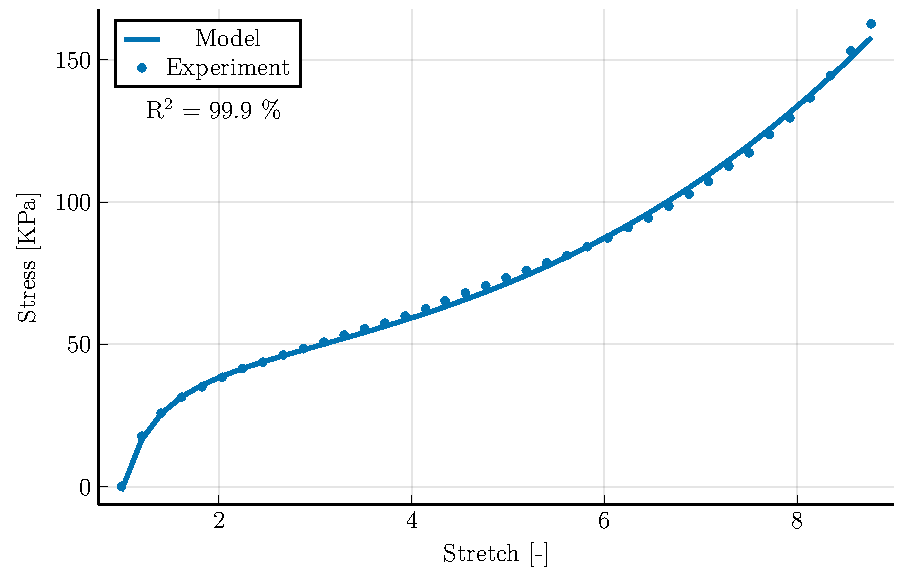
\includegraphics[width=\textwidth]{figures/long_term_characterization.pdf}
    \caption{nonlinear Mooney-Rivlin.}
    \label{fig:long_term_neo_hookean}
  \end{subfigure}
  \hfill
  \begin{subfigure}{0.49\textwidth}
    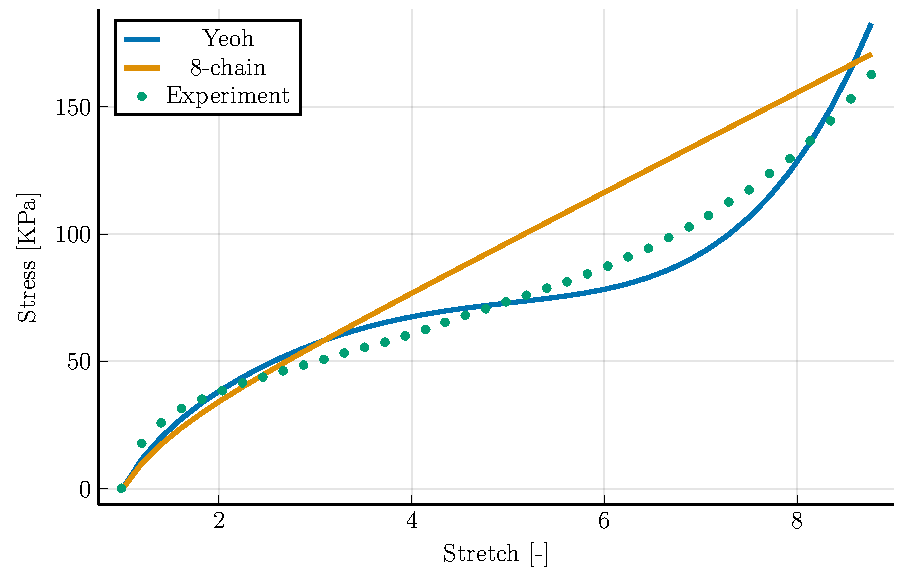
\includegraphics[width=\textwidth]{figures/long_term_comparison.pdf}
    \caption{Hyperelastic models used for comparison.}
    \label{fig:long_term_comparison}
  \end{subfigure}
  \caption{Long-term characterization for the viscoelastic model.}
  \label{fig:long_term_characterization}
\end{figure}


\begin{figure}[htbp]
  \centering
  \begin{subfigure}{0.49\textwidth}
    
\includegraphics[width=\textwidth]{figures/viscous_characterization_stretch.pdf}
    \caption{One-cycle loading-unloading at reference temperature and at fixed loading maximum stretch.}
  \end{subfigure}
  \begin{subfigure}{0.49\textwidth}
    
\includegraphics[width=\textwidth]{figures/viscous_characterization_vel.pdf}
    \caption{One-cycle loading-unloading at reference temperature and at fixed velocity.}
  \end{subfigure}
  \caption{One-cycle loading-unloading tests with the calibrated viscoelastic model.}
  \label{fig:viscous_characterization}
\end{figure}


The sensitivity analysis applied to the viscous model highlights the significance of the number of branches. Multiple characterizations have been performed, from one to four branches, and the results are summarized in table \ref{tab:viscous_characterization}, it can be observed how the $R^2$ fit increases with the number of branches, whereas the sensitivity shows a decay \cite{Cacuci_Uncertainty} for more than three viscous branches. The estimation of the covariance matrix around the optimal parameters $p^*$ allows further exploration of the results, thus, a graphical interpretation of the lower sensitivity can be found in figure \ref{fig:uncertainty_comparison}, where the simulation of a single one-cycle test has been reproduced with 100 sampling models representing the multivariate normal distribution obtained from the covariance matrix \cite{Tarantola_Inverse}.


\begin{table}[htbp]
  \centering
  \caption{Optimal parameters and statistical analysis for the viscous characterization. Units in SI.}
  \label{tab:viscous_characterization}
  \begin{tabular}{cccrrrr}
    \toprule
    Branches & R2 & Parameter & Value & Interval & Error & Sensitivity \\
    \midrule
    \multirow{2}{*}{1} & \multirow{2}{*}{$78\%$}
      & $\mu_1       $ & \num{2.5e+04} & $\pm\num{1.9e+03}$ & $7.6\%$ & 10.2 \\
    & & $\log(\tau_1)$ & \num{    1.9} & $\pm\num{  0.079}$ & $4.1\%$ & 34.7 \\
    \addlinespace
    \cline{3-7}
    \addlinespace
    \multirow{4}{*}{2} & \multirow{4}{*}{$90\%$}
      & $\mu_1       $ & \num{3.5e+04} & $\pm\num{2.9e+03}$ & $8.3\%$ &  8.6 \\
    & & $\log(\tau_1)$ & \num{      1} & $\pm\num{  0.073}$ & $7.2\%$ & 21.6 \\
    & & $\mu_2       $ & \num{9.6e+03} & $\pm\num{6.2e+02}$ & $6.5\%$ & 16.4 \\
    & & $\log(\tau_2)$ & \num{    3.1} & $\pm\num{    0.1}$ & $3.3\%$ & 31.9 \\
    \addlinespace
    \cline{3-7}
    \addlinespace
    \multirow{6}{*}{3} & \multirow{6}{*}{$94\%$}
      & $\mu_1       $ & \num{1.1e+04} & $\pm\num{  2e+03}$ & $18.7\%$ &  5.5 \\
    & & $\log(\tau_1)$ & \num{    1.8} & $\pm\num{   0.14}$ & $ 7.7\%$ & 27.5 \\
    & & $\mu_2       $ & \num{6.6e+03} & $\pm\num{8.3e+02}$ & $12.6\%$ & 10.7 \\
    & & $\log(\tau_2)$ & \num{    3.5} & $\pm\num{   0.18}$ & $ 5.2\%$ & 14.1 \\
    & & $\mu_3       $ & \num{3.7e+04} & $\pm\num{4.5e+03}$ & $12.3\%$ &  3.8 \\
    & & $\log(\tau_3)$ & \num{   0.63} & $\pm\num{   0.12}$ & $19.0\%$ &  4.5 \\ 
    \addlinespace
    \cline{3-7}
    \addlinespace
    \multirow{8}{*}{4} & \multirow{8}{*}{$94\%$}
      & $\mu_1       $ & \num{1.4e+03} & $\pm\num{1.4e+03}$ & $104.5\%$ &  0.5 \\
    & & $\log(\tau_1)$ & \num{    4.1} & $\pm\num{    1.5}$ & $ 35.8\%$ &  0.2 \\
    & & $\mu_2       $ & \num{3.5e+04} & $\pm\num{4.4e+03}$ & $ 12.7\%$ &  7.9 \\
    & & $\log(\tau_2)$ & \num{   0.97} & $\pm\num{    0.3}$ & $ 30.9\%$ & 18.4 \\
    & & $\mu_3       $ & \num{1.2e+03} & $\pm\num{6.7e+03}$ & $549.2\%$ &  0.1 \\
    & & $\log(\tau_3)$ & \num{      2} & $\pm\num{   0.52}$ & $ 25.8\%$ &  0.8 \\
    & & $\mu_4       $ & \num{7.9e+03} & $\pm\num{3.8e+03}$ & $ 48.0\%$ & 10.8 \\
    & & $\log(\tau_4)$ & \num{      3} & $\pm\num{   0.21}$ & $  6.9\%$ & 22.8 \\
    \bottomrule
  \end{tabular}
\end{table}



\begin{figure}[htbp]
  \centering
  \begin{subfigure}{0.49\textwidth}
    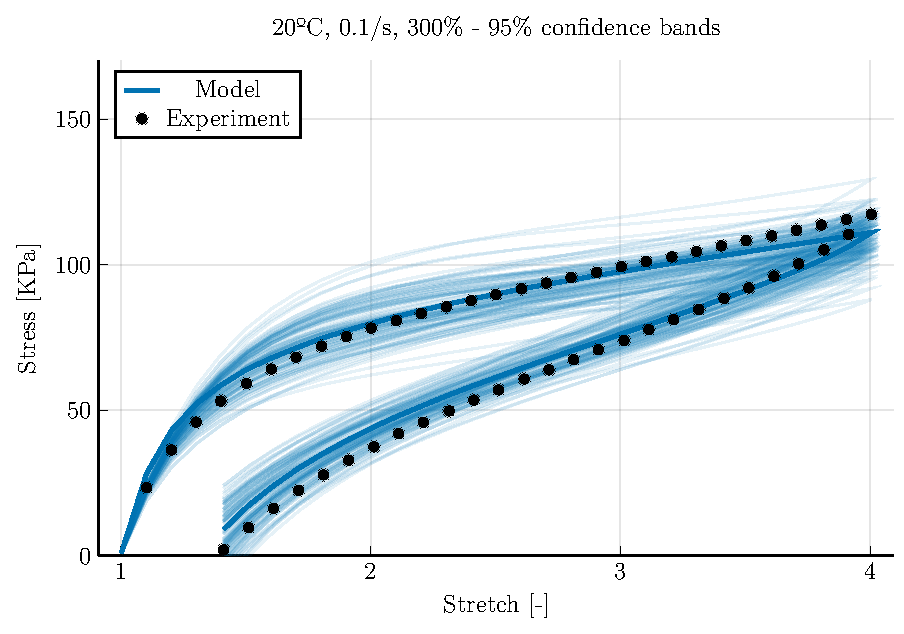
\includegraphics[width=\textwidth]{figures/uncertainity_3_branches.pdf}
    \caption{3 branches}
    \label{fig:uncertainty_3_branches}
  \end{subfigure}
  \hfill
  \begin{subfigure}{0.49\textwidth}
    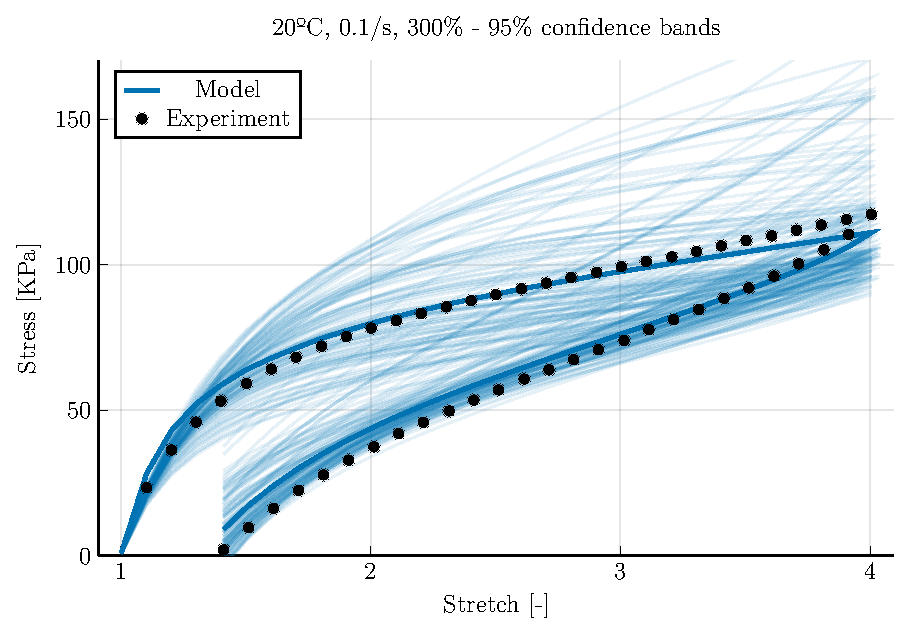
\includegraphics[width=\textwidth]{figures/uncertainity_4_branches.pdf}
    \caption{4 branches}
    \label{fig:uncertainty_4_branches}
  \end{subfigure}
  \caption{Uncertainty quantification of the calibrated model for the viscoelastic testing. Simulation of the one-cycle loading-unloading tests at $20^\circ C$, $0.1/s$ strain rate and $300\%$ maximum stretch.}
  \label{fig:uncertainty_comparison}
\end{figure}


Additionally, the simulation of some experiments are shown in figure \ref{fig:viscous_characterization}, were the ability to predict the experimental results under variations in the strain rate and maximum stretch can be qualitatively observed, showing a satisfactory fit.


\subsubsection{Steps 4 \& 5: Thermo-Mechanical and Electro-Mechanical coupling}

\begin{figure}[htbp]
  \centering
  \begin{subfigure}{0.49\textwidth}
    
\includegraphics[width=\textwidth]{figures/viscous_thermal_laws.pdf}
    \caption{As calibrated}
    \label{fig:viscous_thermal_coupling_laws}
  \end{subfigure}
  \hfill
  \begin{subfigure}{0.49\textwidth}
    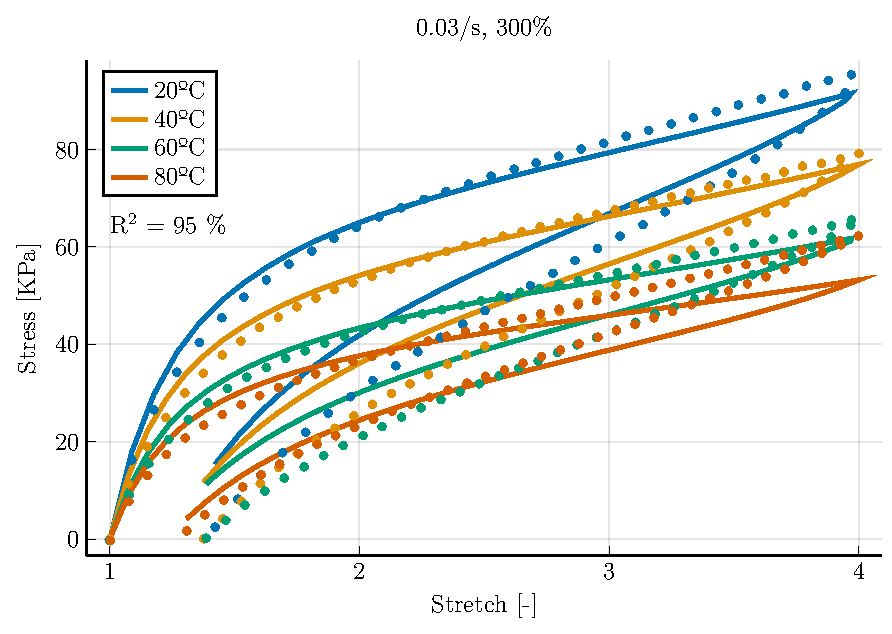
\includegraphics[width=\textwidth]{figures/viscous_fitting_thermal.pdf}
    \caption{$\Psi \time 2$}
    \label{fig:viscous_thermal_coupling_fitting}
  \end{subfigure}
  \caption{Thermo-mechanical coupling. Simulation and experimental data comparison for one-cycle loading-unloading tests.}
  \label{fig:viscous_thermal_coupling}
\end{figure}


The purely thermo-mechanical characterization is closed with the identification of the thermal functions $f_\infty$ and $f_\alpha$. Under the consideration of the sensitivities observed in table \ref{tab:viscous_characterization} and the simple neo-Hookean model for the viscous branches, a single nonlinear softening function \eqref{eqn:thermal_function_f_softening} has been chosen to model viscous coupling with the temperature. As for the long-term component, the authors in \cite{Dippel2015, Liao_Mokarram2020} report very low thermal variation, this observation has motivated the choosing a nonlinear melting function \eqref{eqn:thermal_function_f_melting} because of its smooth changes around the reference temperature. The melting point has been considered $\theta_M=\qty{150}{\degreeCelsius}$, according to the technical specifications \cite{3MVHB4910}.


\begin{table}[htbp]
  \centering
  \caption{Optimal parameters and statistical analysis for the thermal coupling of the viscoelastic constitutive model. Units in SI ($K$).}
  \label{tab:viscous_thermal_coupling}
  \begin{tabular}{crrrr}
    \toprule
    Parameter & Value & Confidence interval & Relative error & Sensitivity index \\
    \midrule
    $\gamma_\infty$ & \num{   0.57} & $\pm\num{ 0.34}$ & $59.5\%$ &    0.1 \\
    $\gamma_\alpha$ & \num{     17} & $\pm\num{  1.5}$ & $ 9.0\%$ &    1.5 \\
    $\theta_T     $ & \num{    310} & $\pm\num{    1}$ & $ 0.3\%$ &  103.5 \\
    $\delta       $ & \num{   0.43} & $\pm\num{0.014}$ & $ 3.3\%$ &   10.5 \\
    \bottomrule
  \end{tabular}
\end{table}


The thermo-mechanical model is closed with the electrical coupling, whose optimal parameters can be found in table \ref{tab:thermo_elec_characterization}. The smooth change of the dielectric permittivity depending on the temperature has been modelled with a nonlinear melting as described in \eqref{eqn:thermal_function_f_melting}, where the degradation temperature $\theta_M$ is not known a priori and it has been included as a parameter to be identified. High sensitivities can be observed in table \ref{tab:thermo_elec_characterization}, however, the parameter $\gamma_\varepsilon$ has lower observability.

\begin{table}[htbp]
  \centering
  \caption{Optimal parameters and statistical analysis for the thermo-electrical characterization. Units in SI.}
  \label{tab:thermo_elec_characterization}
  \begin{tabular}{crrrr}
    \toprule
    Parameter & Value & Confidence interval & Relative error & Sensitivity index \\
    \midrule
    $\epsilon_r        $ & \num{    4.7} & $\pm\num{  0.071}$ & $  1.5\%$ & 130042.9 \\
    $\gamma_\varepsilon$ & \num{      3} & $\pm\num{    8.4}$ & $285.4\%$ &    355.1 \\
    $\theta_M          $ & \num{    570} & $\pm\num{4.4e+02}$ & $ 77.1\%$ &   5029.3 \\
    \bottomrule
  \end{tabular}
\end{table}



\subsubsection{Step 6: Model Validation}

Finally, two types of validation have been performed, a comparison against the fully coupled thermo-electro-mechanical experimental data, and a validation of the positivity of the specific heat. In figure \ref{fig:fully_coupled_experim}, four fully coupled loading-unloading tests have been reproduced and compared against experimental data reported in \cite{Mehnert2021a}. This is a blind validation, where the dataset is independent from the data used for the calibration. It can be noted that the negative values near the non stretched configuration are compatible with the experimental data and the kinematics in \eqref{eqn:F_thermo_electro_mech}.


\begin{figure}[htbp]
  \centering
  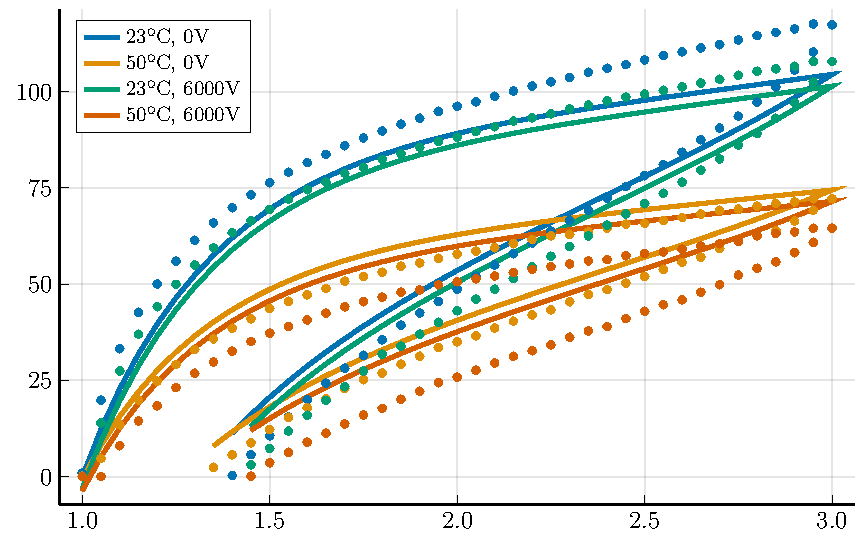
\includegraphics[width=0.60\textwidth]{figures/fully_coupled_experiments_0.pdf}
  \caption{Reproduction of thermo-electro-mechanical tests with the calibrated model.}
  \label{fig:fully_coupled_experim}
\end{figure}



\paragraph{Kinematic Generalization and Hyperelastic Model Transition}
\label{sec:model_transition}

While the invariant-based modified Ogden model developed in Section \ref{sec:constitutive equations} provides an exceptional descriptive capability for the uniaxial experimental spectrum—achieving a remarkably high adjusted $R^2$—a critical transition is required when moving from one-dimensional characterization to multi-dimensional boundary value problems. 

During electro-mechanical actuation, the electrostatic Maxwell stress compresses the material through its thickness, kinematically forcing an in-plane, equal-biaxial expansion. Consequently, the local deformation state within a fully coupled 3D continuum is characterized by a complex superposition of uniaxial tension and biaxial extension. It is well recognized in rubber elasticity that hyperelastic formulations utilizing the second invariant $I_2$ are highly sensitive to data limitations; when calibrated strictly on uniaxial datasets, their extrapolation to multi-axial deformation states frequently triggers material instabilities or unphysical softening. 

To ensure mathematical stability and predictive robustness in the subsequent finite element simulations, the $I_1$-based Yeoh model is selected for the numerical applications. Although the Yeoh model exhibits a lower adjusted $R^2$ during the uniaxial calibration phase due to its simpler invariant structure, its dependence solely on $I_1$ inherently safeguards it against the wild extrapolative errors typical of $I_2$ models. This transition represents a deliberate, physically motivated trade-off: sacrificing a minor degree of statistical accuracy in a pure 1D tension fit to guarantee robust, qualitatively sound, and unconditionally stable predictive capabilities across complex, multi-axial electro-thermo-mechanical loading scenarios.



\paragraph{Thermodynamic consistency and specific heat post-computation}


\begin{figure}[htbp]
  \centering
  \begin{subfigure}{0.49\textwidth}
    
\includegraphics[width=\textwidth]{specific_heat_post_computation_0.pdf}
    \caption{Model with non-compliant thermodynamic coupling.}
    \label{fig:specific_heat_computation_0}
  \end{subfigure}
  \hfill
  \begin{subfigure}{0.49\textwidth}
    
\includegraphics[width=\textwidth]{specific_heat_post_computation.pdf}
    \caption{Model with the presented thermal coupling.}
    \label{fig:specific_heat_computation}
  \end{subfigure}
  \caption{Theoretical specific heat capacity computed at the maximum stretch of multiple experiments. Each 2D point represents a one-cycle loading-unloading test. The thick rectangle identifies the region explored by the experimental data.}
\end{figure}


% \subsection{Conclusions}

% First of all, in order to perform a consistent calibration of the constitutive model presented in \ref{sec:constitutive equations}, only a few experimental data has been selected among the literature (see tables \ref{tab:experiment_sources} and \ref{tab:calibration_steps}) because of the big discrepancies of reported values for the same experiment under the same conditions among different laboratories, and the need to isolate the uncertainty from data acquisition and the uncertainty inherent to the limitations of the constitutive model. Even though, data from three different research groups has been combined for the calibration and the overall result has proven to be accurate.

% The calibration of the thermally-coupled volumetric energy, even if the variation of the specific heat capacity is almost linear \cite{Dippel2015}, has demonstrated to be consistent in terms of energy, entropy and specific heat capacity. Furthermore, an indirect characterization of the bulk modulus $\kappa_R$ has been performed and it is in good agreement with standard values.

% Regarding the deviatoric response of the material, it has proven to be more accurate to perform a staggered characterization of the long term component and the viscous branches. From the numerical optimizations, different optimal parameters had been observed if a monolithic calibration would be performed. Additionally, models that depend solely on the first invariant $I_1$, do not seem to accurately capture the the response of the material, for that reason, a nonlinear Mooney-Rivlin model has been chosen. For the sake of simplicity, the viscous branches are modelled with simple neo-Hookean models, however, the choice of a more complex model would easily enhance the fitting, at the cost of increasing the number of parameters.

% The observation of the error metrics such as the sensitivity index for each calibrated parameter had allowed a quantitative criterion the choose the number of viscous branches. Three branches provide the best fitting, even two viscous branches with a neo-Hookean model provide good results, adding a fourth branch would result into an overfitted model.

% With regard to the thermoelasticity coupling, each component of the free energy density has been modelled with an independent thermal law, a nonlinear softening has been proposed, as a direct extension of the model presented in \cite{BonetGil2026}. Due to statistical observability, all the viscous branches have been modelled with the same thermal function.

% Finally, two types of validation have been performed. The calibrated model was used to reproduce the thermo-electro-mechanical experiments presented in an independent publication, offering a blind validation with a fitting $R^2=93\%$. additionally, the specific heat capacity has been computed for different combinations of stretch and temperature, to validate the positivity of the specific heat and fulfilment of the third law of the thermodynamics.



